\documentclass[a4paper]{jpconf}
\usepackage{graphicx}
\bibliographystyle{iopart-num}
\usepackage{citesort}

\begin{document}
\title{Optimization and performance measurements of ROOT-based data formats in the ATLAS experiment}

\author{Ilija Vukotic for the ATLAS collaboration}

\address{Laboratoire de l'Acc\'{e}l\'{e}rateur Lin\'{e}aire, Universit\'{e} Paris-Sud 11, B\^{a}timent 200, 91898 Orsay, France}

\ead{ivukotic@cern.ch}

\begin{abstract}
  The interplay of the ATLAS persistent event data model and the ROOT based I/O backend was studied in order to improve the read performance and disk size of ATLAS data formats for simulation, reconstruction and data analysis.  The enabling of several native ROOT features, such as basket ordering and the tree cache, has lead to significant improvements in dedicated test setups using local disks, file servers managed by dCache, DPM, and xrootd.  After implementation in the ATLAS Athena framework, tests in more realistic environments were done. The functionality of the improvements and results from the performance tests are reported.
\end{abstract}

\section{Introduction}

ATLAS~\cite{atlas} is recoding RAW data at up to 450 MB/s and at the time of writing (December 2010) has already collected 45 pb$^{-1}$ ($3.2\times10^{12}$ events) at 7 TeV center of mass energy proton-proton collisions. In addition 1.25 times as much of the derived data formats has been produced (not counting Monte Carlo data). Data analysis is also intensifying and is currently performed at more than 70 sites by an average 1000 users, which submit more than 16~000 jobs per day.
With this much data to store and analyze it is of utmost importance to have minimal file size and optimal IO performance across different usage paterns and storage technologies.

\section{Data}
For this study we used only ESD (event summary data - contains full reconstruction information), AOD (analysis object data - subset of ESD objects and primary analysis format ) and D$^3$PD (derived physics data) formats. Summary of data size, even size, and number of root branches is given in table~\ref{table_datasets}. D$^3$PD files contain just two trees with simple variables and vectors of simple variables, so all the information is available directly from ROOT~\cite{root}. AOD and ESD formats are produced using POOL RootStorageSvc \footnote{POOL is a part of the LCG persistency framework and  provides technologically neutral object persistency with navigational capabilities} and their structure is considerably more complex. To reduce the storage space needs as much as possible, we do not store objects as they are reconstructed but we first convert them to their "persistent" representation. The conversion procedure frequently drops part of the member variables, reduces precision and in some cases employs prior knowledge to compress data. The conversion framework also provides a way for storage format independent schema evolution. Converters of most of the composed objects call in turn converters corresponding to their non-simple members. For some objects (e.g. TrackCollection) this can mean that up to 20 different converters are called to store them.
Detailed description of data formats, their production and usage may be found in~\cite{Karsten}.
\begin{table}[h]
\caption{\label{table_datasets}Details on datasets used.}
\begin{center}
\lineup
\begin{tabular}{ lllll  }
	\br
	format & files & size & event size & branches \cr
           &        & [GB] & [kB/event] &  \cr
	\mr
	AOD           & \0274   & \0834 & \0129.44 & 10532 \cr
	ESD           & 3408    & 8784 & 1363.09 &  15734 \cr
	NTUP\_EGAMMA  & \0532   & \0\092 & \0\014.22 & \02383\cr
	MC ESD        & \0\0\01 & \0\0\00.90 & 1887.85 & 13993\cr
	MC ADO        & \0\0\01 & \0\0\00.27 & \0559.91 & \09956\cr
	\br
\end{tabular}
\end{center}
\end{table}


\section {Single file tests}

To be able to understand the results of the large scale tests we start with single file read tests. Two types of single file tests have been performed. The first one where the file is already cached in memory by the operating system and thus provide us with pure CPU read times and the second one where we make sure no part of the file is in the memory thus gives us total wall-clock read time. 

\subsection{CPU only times}

Pure CPU read times are summarized in table~\ref{table_CPUtimes}. Data were read using Athena~\cite{athena}, and times where measured using ChronoSvc of Gaudi framework~\cite{gaudi}. In this table, root speed column represents the time it takes for root to "read" the data, unzip the branches and create our persistent objects. Total speed column also includes the time needed to convert persistent to transient objects. (Our goal is to have the total read CPU time not more than  10-20\% longer than the root time) Large difference in both root and total speeds can be attributed to the fact that different collections are stored in different file formats in combination with their very different read speeds. This can easily be seen from figure~\ref{fig_AOD_R}. We store more than 300 collections and most of them are very small (less than few kB/event). We observe that root read speed decreases with the object size and with increase of complexity (the number of branches in a collection).

\begin{figure}[htbp]
\begin{center}	
\leavevmode
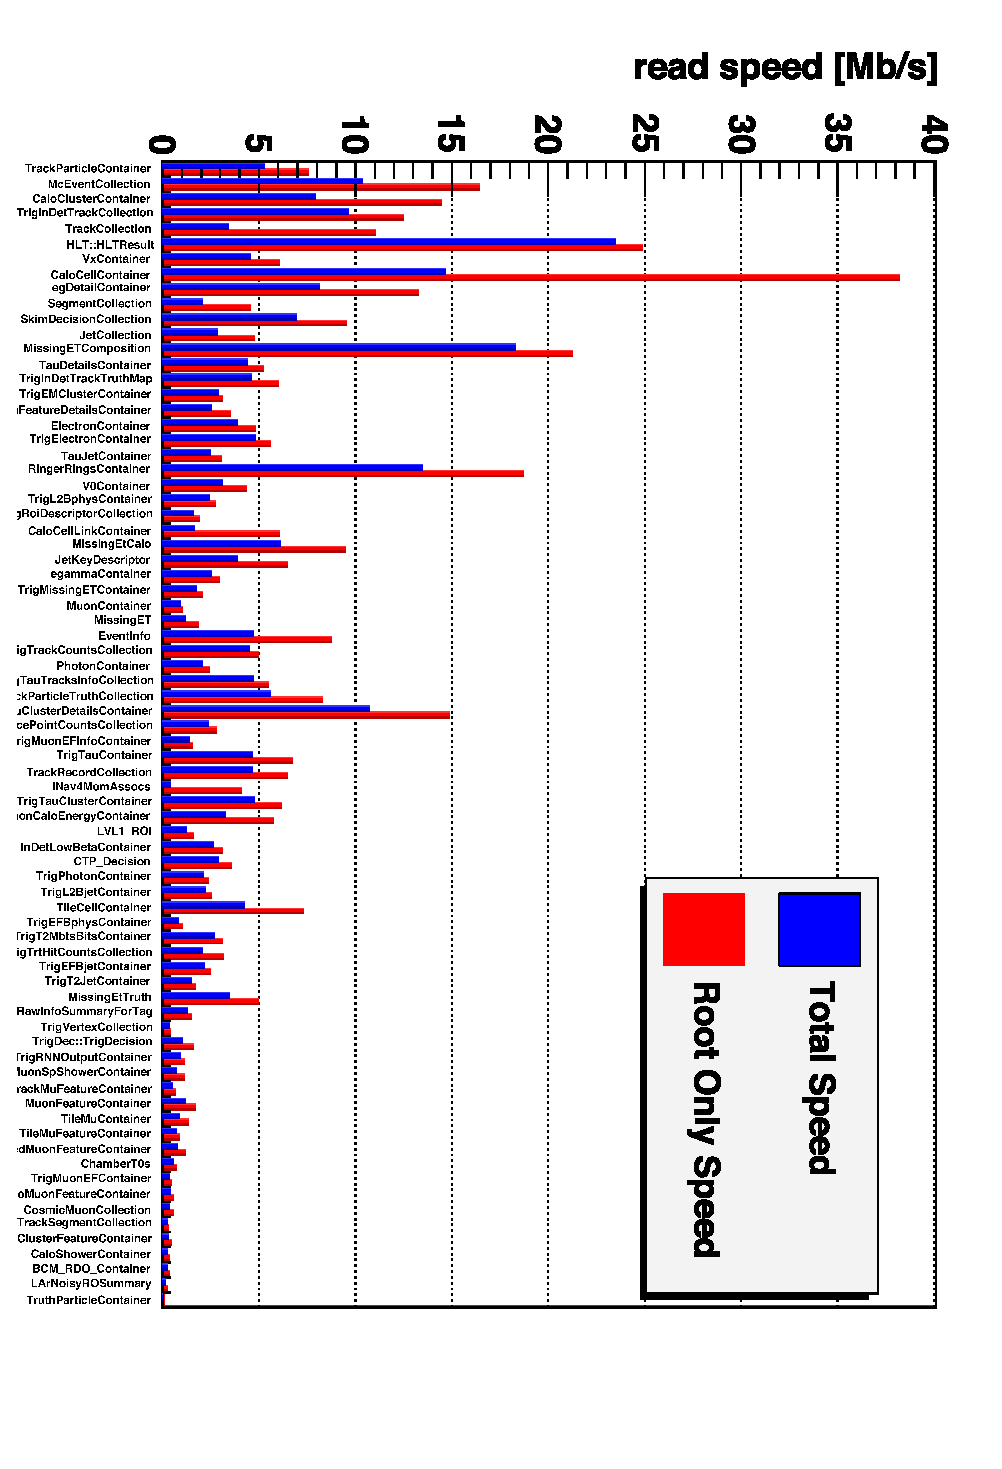
\includegraphics[scale=0.65, angle=90]{AOD_R_speed_manual_edit}
\end{center}
\caption{Different collections show very different read speeds. Large and simple collection show the largest ROOT only speeds. Collections are ordered by size which decreases from left to right.}
\label{fig_AOD_R}
\end{figure}


\begin{table}[h]
\caption{\label{table_CPUtimes}Measured pure CPU read speeds using Athena. Total speed includes time spent in t/p conversion. }
\begin{center}

\lineup
\begin{tabular}{ lll }
	\br
	format & root speed & total speed\cr
	       & \0\0[MB/s] & \0\0[MB/s] \cr
	\mr
	MC - AOD   & \0\0\0\08.38 & \0\0\05.20 \cr
	MC - ESD   & \0\0\012.99 & \0\0\03.69 \cr
	real - AOD & \0\0\0\02.36 & \0\0\01.60\cr
	real - ESD & \0\0\0\09.42 & \0\0\03.22\cr
	\br
\end{tabular}
\end{center}
\end{table}


\subsection{Local disk results}
To understand real (wall-clock) time and some possibilities for improvement, it is important to know how root stores data. Object members are streamed into their own buffers (baskets). These are written to file as soon as they get full. As it may be inferred from figure~\ref{fig_ROOT_storage} this leads to the situation where in order to read one full event one has to read its parts from the different positions in the file. Frequent jumps through the file lead to an increase in wall-clock read time and all of the optimizations try to reduce their number. The optimization problem is further complicated by multiple read patterns: full data, some events, parts of events, and in the case of D$^3$PD files reading by PROOF~\cite{proof}.

\begin{figure}[h]
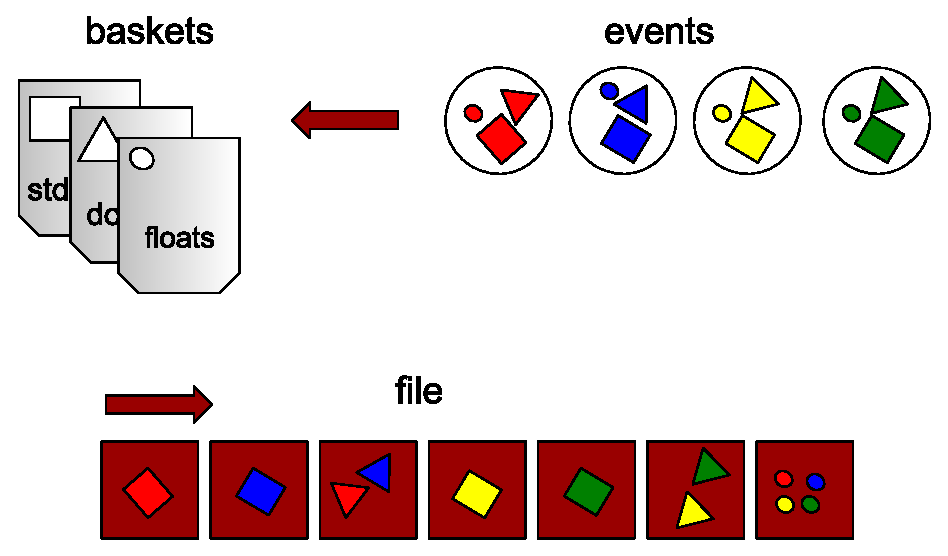
\includegraphics[width=17pc]{ROOT_storage.eps}\hspace{2pc}%
\begin{minipage}[b]{17pc}\caption{\label{fig_ROOT_storage}Object members are streamed into their own buffers which are written to file as soon as they get full. Parts of the same event end up at different positions in the file}
\end{minipage}
\end{figure}
  
Simplification of the persistent data model is one of the obvious optimization methods we use, but it requires manpower which happens to be our scarcest resource. Basket size, zip level, and split level are three of the root settings that simultaneously influence disk size, IO memory footprint, and read speed. We find that baskets of 2 kB for all branches, zip level 6, and full split (level 99) are optimal for our data.
Using TTreeCache when reading the files reduces read time by ordering and predicting read requests but introduces one more memory buffer. 
Two more optimization options are to reorder the baskets which can be made according to event(entry) number or according to branch.
All ATLAS files produced at Tier0 are re-ordered by event.
Finally starting with Athena 15.9.0, which uses root 5.26.00.d, we have a possibility to use the root autoFlush functionality. This works in the following way: the first time that a preset amount of data has been collected (by default 30 MB) the sizes of baskets are optimized and their content is written to file. The next flush to file happens when the same number of events has been written.

Wall-clock times from tests on reading a single AOD file from local disk are shown at figure~\ref{fig_LOCAL_AOD}. Moving from unordered files at the beginning of the data taking to the ordered ones we use now, improved our read speed by more than a factor of 3. Using TTreeCache proved to be beneficial in sparse read scenarios. While ROOT optimized AOD files showed a clear advantage over simple reordered AOD files in all the scenarios, in the case of reading all of the ESD events, the opposite was observed. All the read scenarios on D$^3$PD files show that unordered files, with or without TTreeCache, performed the worst, while ROOT optimized files were the fastest. 

\begin{figure}[h]
\begin{center}	
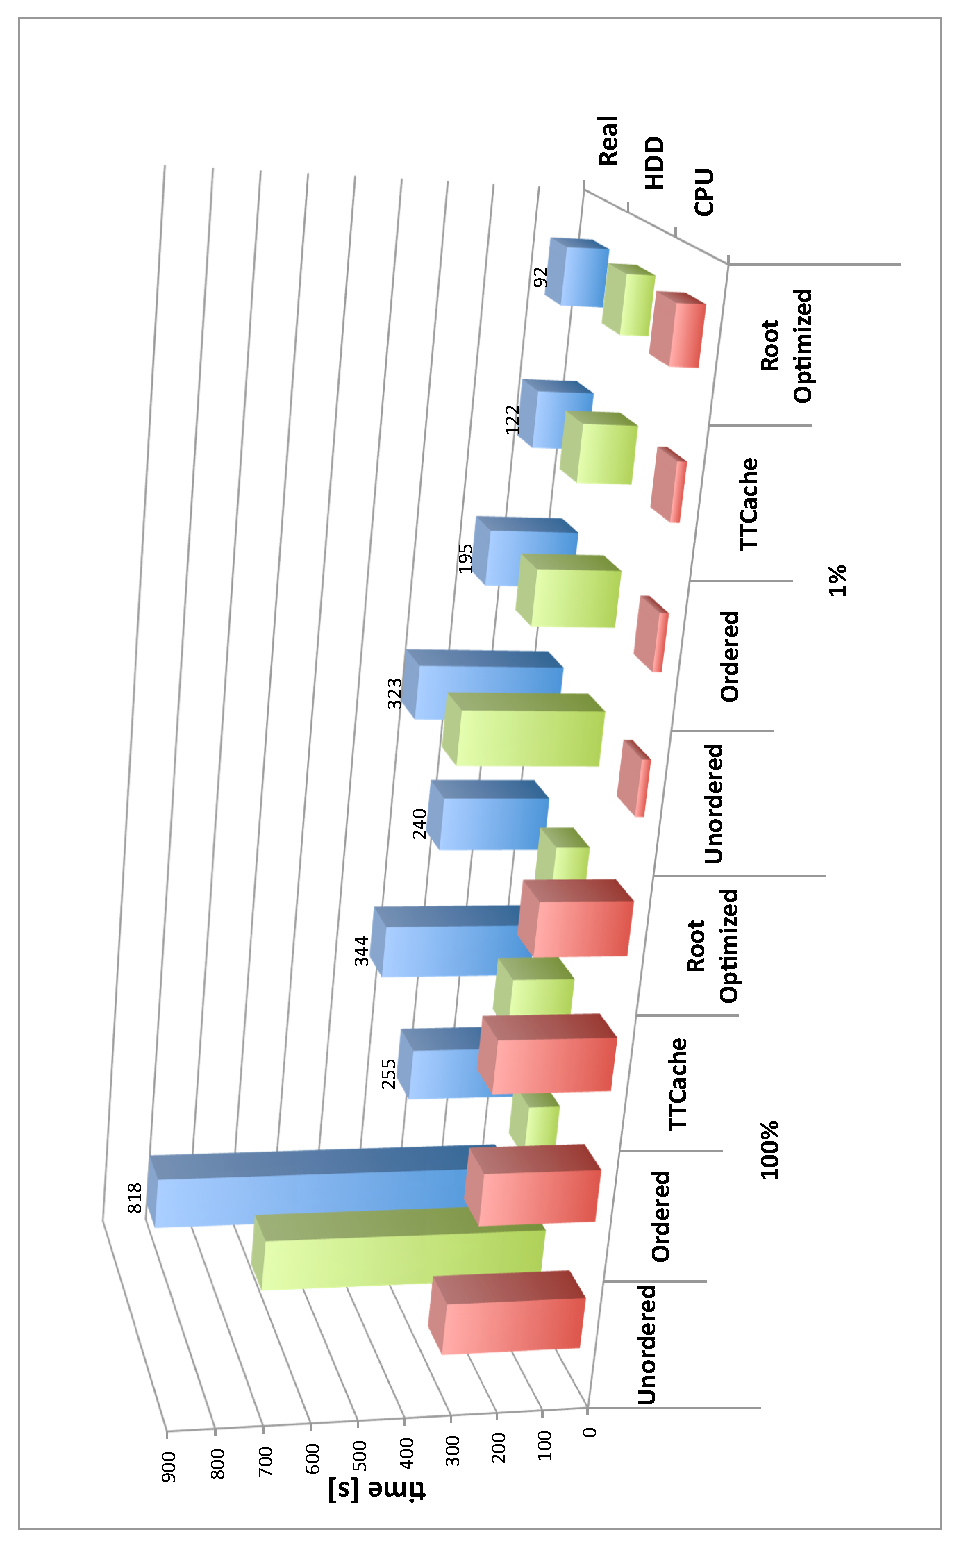
\includegraphics[scale=0.5, angle=-90]{LOCAL_AOD.eps}
\end{center}
\caption{\label{fig_LOCAL_AOD}AOD read performance from local disk. }
\end{figure}



\section{Large scale tests}

At Laboratoire de l'Acc\'{e}l\'{e}rateur Lin\'{e}aire, Orsay, a dedicated farm with 80 cores running scientific linux 5 was established for the IO performance tests. As a backend, a DPM~\cite{dpm} storage element has been used.  Three tests reading all the AOD data using Athena were performed. When reading original(unordered) files we observe 85\% CPU utilization, and it appears that jobs are disk seek speed bound giving a total wall-clock running time of 9h 30min. Reading ordered files was CPU bound, and jobs took 5h 35min. Reading original files, but with a TTreeCache of 20MB switched on, we observe a running time of 4h 34min with a CPU occupancy of 92\%.     

Reading D$^3$PD files using PROOF via DPM/xrootd~\cite{xrd} plugin showed big performance issues and for that reason we will not quote any result from these tests. DPM was never before used in this way but since major problems are already identified, we expect the new version to address them. 

DPM was again tested in Glasgow this time with a rfio plugin. Results are compared to the ones from Lustre~\cite{lustre} file system at Queen Mary, University of London. Results of single file read tests are shown in figure~\ref{fig_DPM_LUSTRE}. The DPM default setting uses 1MB of read-ahead cache as it gives the best performance for jobs pre-staging data. This was giving very bad performance in all test cases. Reducing the cache size to 4kB gave much better times, which are almost the same across all the tests. It is interesting to notice that Lustre shows significantly better results for ordered files when used together with TTreeCache than without it. We still lack an explanation of this effect.

\begin{figure}[h]
\begin{center}	
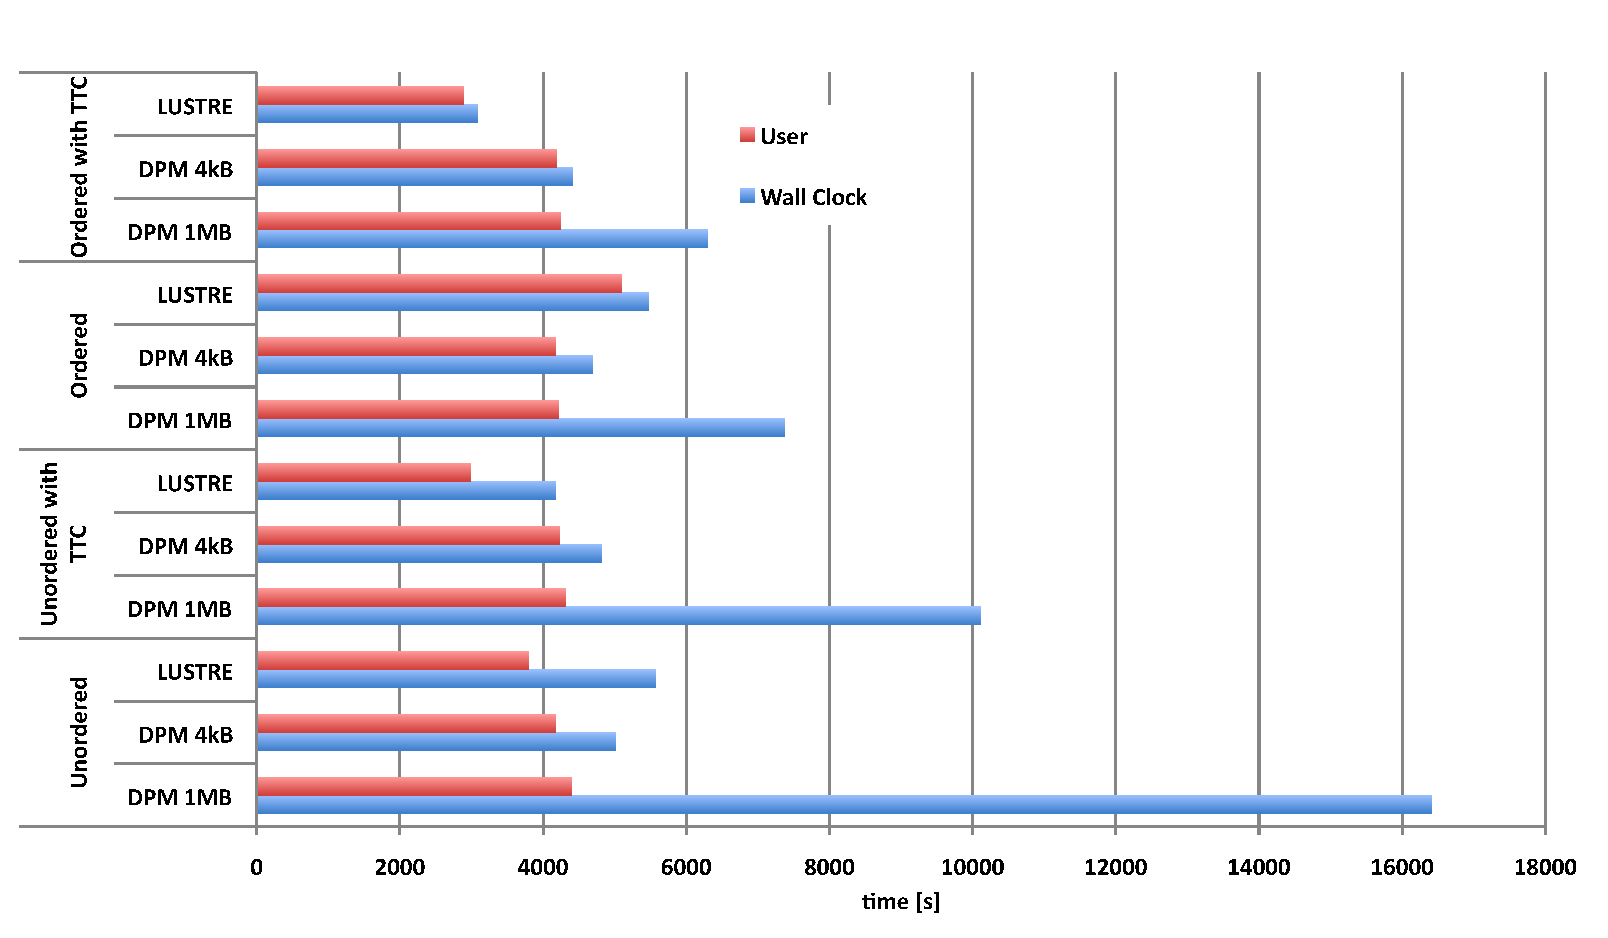
\includegraphics[scale=0.6]{wahid.eps}
\end{center}
\caption{\label{fig_DPM_LUSTRE}Comparison DPM/rfio and Lustre. }
\end{figure}

Both systems scaled well when tested on the full ordered dataset. DPM/rfio showed 88\% and 93\% CPU efficiencies without and with TTreeCache respectively. Corresponding Lustre numbers are 77\% and 93\%.   

We had an opportunity to perform a few tests on EOS~\cite{EOS}, a xroot-managed disk pool prototype that is under consideration for analysis-style data access at CERN. This xroot server comprises 24 nodes with twenty 2TB raid0 file systems each, but we used only 10 of them thus having maximal theoretical throughput of 1~GB/s. Load was provided by 23 eight core machines running ROOT 5.26.0b (slc4, gcc 3.4) organized in a PROOF cluster and reading the D$^3$PD dataset.
As it may be seen from figure~\ref{fig_EOS} when reading sequentially all the events of the optimized dataset we observed rates of 32.000~events/s which corresponds to 550~MB/s and were CPU bound. Read rate of the unoptimized data set was disk bound. Sparse reading of the randomly distributed 1\% of events shows very bad performance. In the case of unoptimized files we could read at most 90 selected events per second. This is worse than reading all of the events and just discarding the unneeded ones, which would give us 127~events/s. The situation is somewhat better with optimized files but still far from acceptable.  

\begin{figure}[h]
\begin{center}	
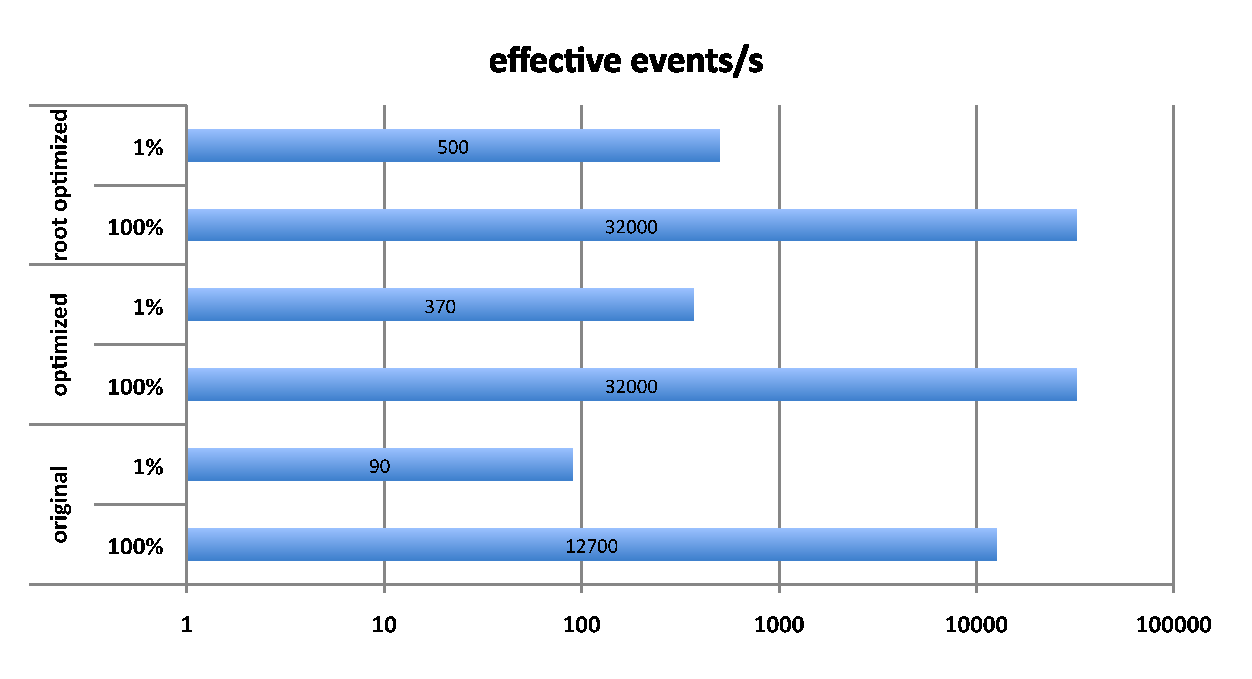
\includegraphics[scale=0.6]{EOS.eps}
\end{center}
\caption{\label{fig_EOS}PROOF cluster reading full D$^3$PD dataset from EOS. Shown are maximal sustained event rates.}
\end{figure}

dCache~\cite{dcache} was tested and compared to Lustre at NAF(German National Analysis Facility) centers in Hamburg and Zeuthen. Tests were running real analysis codes used for the first ATLAS results from minimum bias data. Both unoptimized (ROOT 5.22) and optimized (ROOT 5.26, compression level 2) D$^3$PD data sets were used. Once again we see a clear advantage in using optimized files, but here dCache showed significantly worse results than Lustre. Only 20 jobs were enough to completely saturate dCache at rates of less than 1GB/s.

\section{Conclusion}
The volume of data produced by the ATLAS experiment makes their efficient reading extremely important. In the quest of improving it, there are many possible ways and parameters to optimize. Several different file formats and use cases with sometimes conflicting requirements make optimization more difficult. The currently used file reordering significantly decreased job duration and stress on the disk systems. Further improvement is expected by enabling new root features like basket size optimization and autoFlush.
All of the tested storage backends DPM, Lustre, xroot, and dCache need careful job specific tuning to reach optimal performance. Even using strong hardware platforms tuned to our needs, efficient data analysis will continue to depend on multi-stage event and/or event size reduction.


\section*{References}
\bibliography{ivukotic_CHEP2010}
  

\end{document}


